\paragraph*{Historical and layer-wise attention structure.}
Figures~\ref{fig:attn-temporal}--\ref{fig:attn-horizons} examine temporal context within the same supplementary mixed-condition analysis. Figure~\ref{fig:attn-temporal} covers all 30 historical windows under normal and upcoming conditions, with an upcoming-minus-normal panel that resolves smaller shifts in the historical positions receiving attention. Its difference scale is much narrower than the absolute-weight scale, so the panel should not be read as a large change in temporal dependence. Figure~\ref{fig:attn-layers} focuses the main-text comparison on encoder layers 1, 4, and 5, retaining an input-near layer and the final two layers while keeping both geographic and semantic branches readable. The complete five-layer view is retained in Appendix~\ref{app:layerwise-attention}. Layer-specific weights do not measure the accuracy contribution of each layer.

Figure~\ref{fig:attn-horizons} compares the upcoming-minus-normal resource maps from three separately trained Start$\leq5/10/15$ mixed-condition checkpoints, with 96 samples per condition and checkpoint. The persistent structure and localized changes provide a descriptive view across onset settings. They neither trace propagation through physical time nor replace the distance-resolved recall comparison in Table~\ref{tab:delay-ablation-new}.

\begin{figure*}[t]
\centering
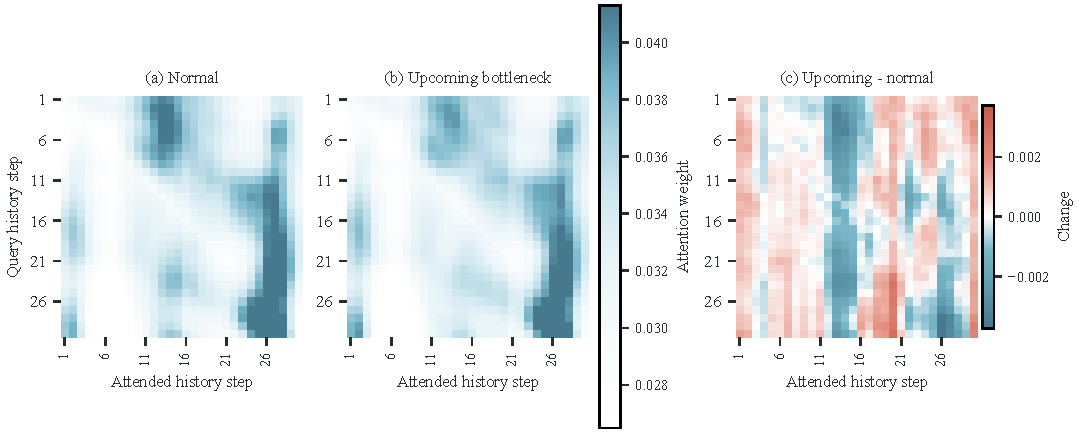
\includegraphics[width=0.98\textwidth]{figures/attention_heatmaps/fig04_temporal_attention_states.pdf}
\caption{Temporal attention over 30 history windows: (a)~normal; (b)~upcoming; (c)~upcoming-minus-normal.}
\label{fig:attn-temporal}
\end{figure*}
\begin{figure*}[t]
\centering
\includegraphics[width=0.92\textwidth]{figures/attention_heatmaps/fig05_layerwise_upcoming_attention_selected.pdf}
\caption{Geographic (upper) and semantic (lower) attention in selected encoder layers 1, 4, and 5.}
\label{fig:attn-layers}
\end{figure*}
\begin{figure*}[t]
\centering
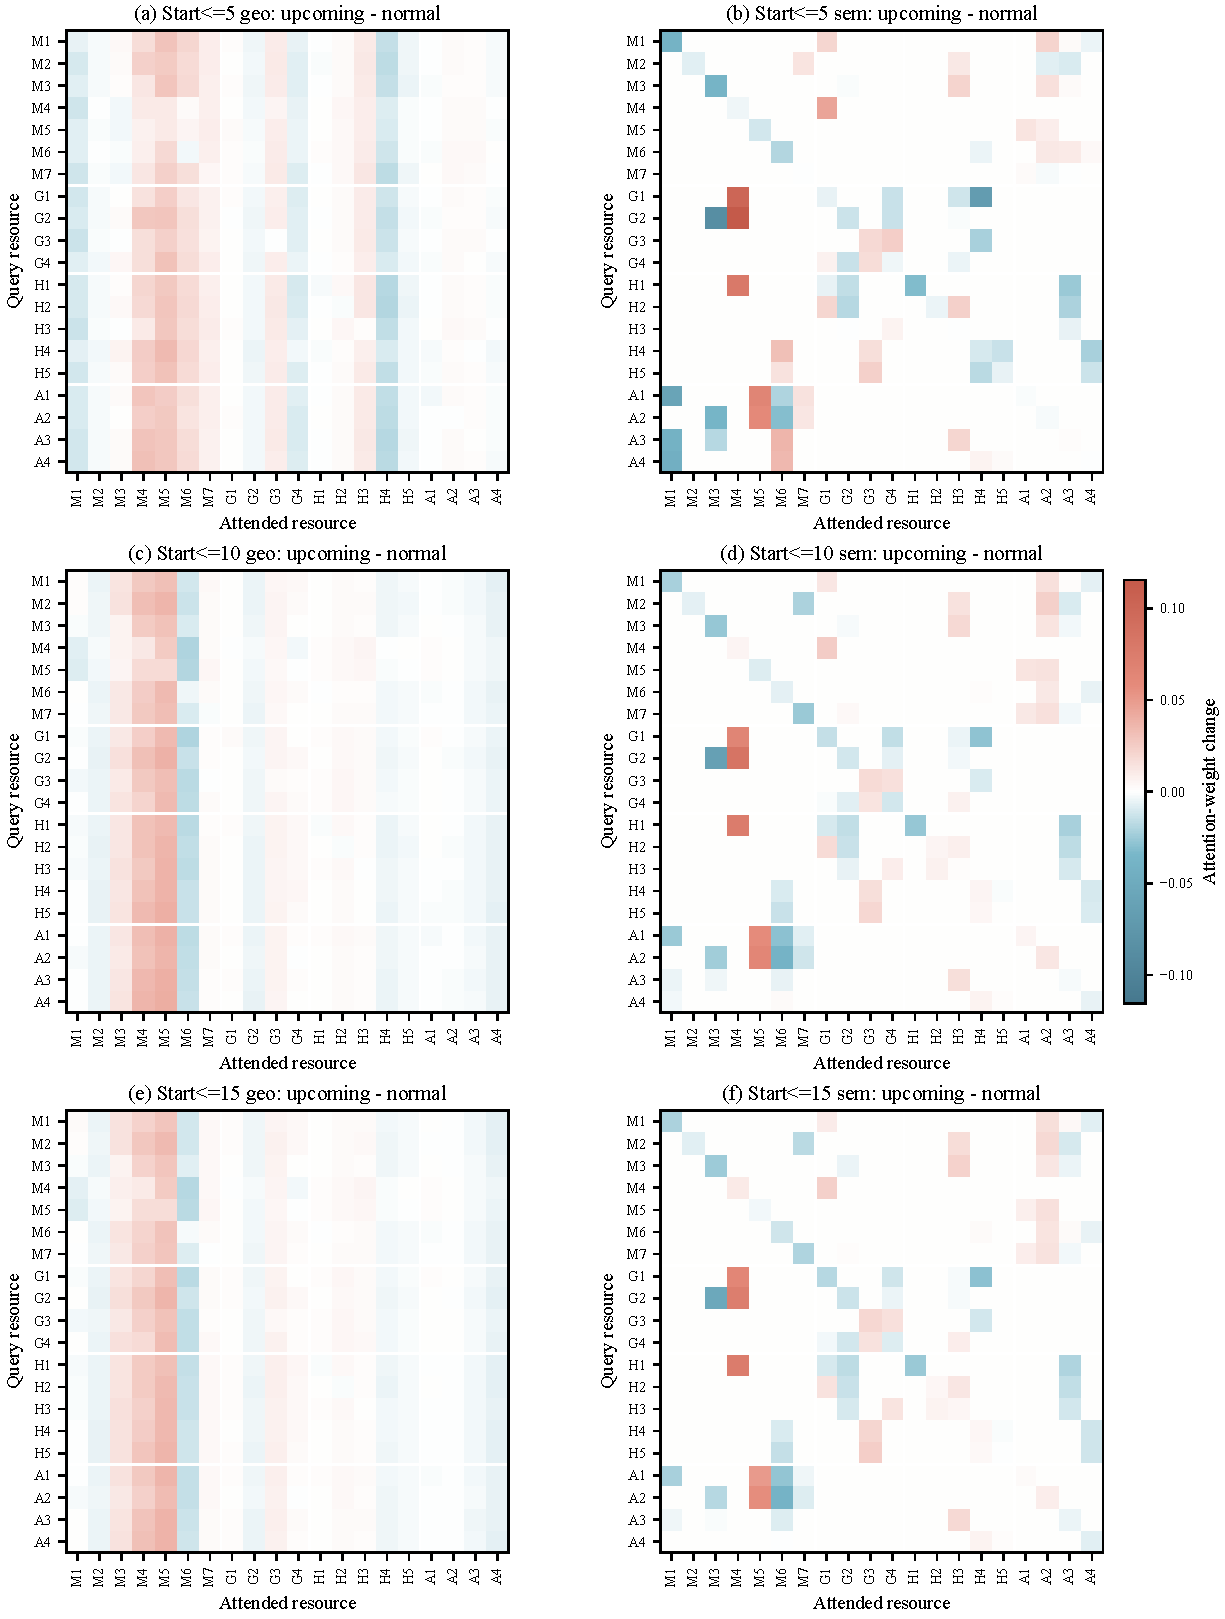
\includegraphics[width=0.98\textwidth]{figures/attention_heatmaps/fig07_horizon_attention_change.pdf}
\caption{Upcoming-minus-normal attention change across Start caps 5/10/15 (upper: geographic; lower: semantic).}
\label{fig:attn-horizons}
\end{figure*}
